

\begin{frame}[t,allowframebreaks]{
    Local minima -}

    A convex \index{optimisation}\gls{optimisation} 
    problem is reduced to finding a 
    \index{local minimum}\gls{local minimum}.
    \begin{itemize}
        \item A \gls{local minimum} is guaranteed to be a
        \index{global minimum}\gls{global minimum}.\\
    \end{itemize}

    \vspace{0.1cm}

    \index{neural network}\Glspl{neural network} with non-linear 
    \index{activation function}\glspl{activation function}
    yield a nonconvex \index{loss function}\gls{loss function}.\\
    \vspace{0.1cm}

    A nonconvex function, 
    can have multiple \glspl{local minimum}.

    \begin{columns}[t]
        \begin{column}{0.40\textwidth}
            \begin{center}
                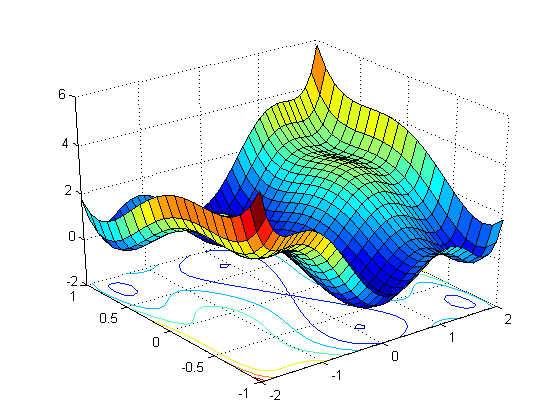
\includegraphics[width=0.98\textwidth]
                    {./images/training_issues/local_minima_illustration.png}\\
                {\tiny 
                    \color{col:attribution} 
                    Taken from \cite{StackExch:MultipleMinima}.\\    
                }
            \end{center}                        
        \end{column}
        \begin{column}{0.60\textwidth}
        \end{column}
    \end{columns}

\end{frame}